%
% zykloide.tex
%
% (c) 2024 Prof Dr Andreas Müller
%
\begin{figure}
\centering
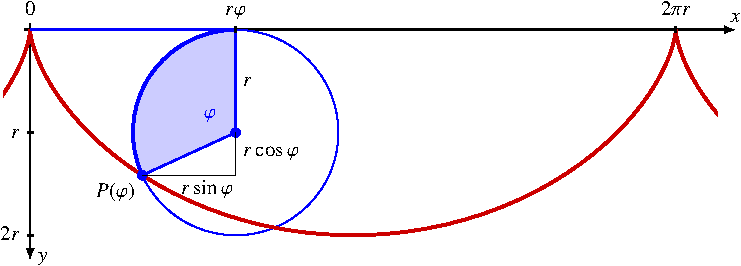
\includegraphics{chapters/020-variation/images/zykloide.pdf}
\caption{Parametrisierung der Zykloide, die durch Abrollen eines
Kreises mit Radius $r$ auf der $x$-Achse entsteht.
Für $t=0$ berührt der Kreis die $x$-Achse im Nullpunkte.
\label{buch:variation:problem:fig:zykloide}}
\end{figure}
